\chapter{Introduction}
\label{ch:cryo-intro}
%% Intro shared by all subsections

\section{An International Physics Program}

The global neutrino physics community is developing a multi-decade
physics program to measure unknown parameters of the Standard Model of
particle physics and search for new phenomena.  The program will be carried out as an international,
leading-edge, dual-site experiment for neutrino science and proton decay studies, which 
is known as the Deep Underground Neutrino Experiment (DUNE).
The detectors for this experiment will be designed, built, commissioned and operated by the international DUNE Collaboration. The facility required to support this experiment, the Long-Baseline Neutrino Facility (LBNF), is hosted by Fermilab and its design and construction is organized as a DOE/Fermilab project incorporating international partners. Together LBNF and DUNE will comprise the world's highest-intensity neutrino beam at Fermilab, in Batavia, IL, a high-precision near detector on the Fermilab site, a massive liquid argon time-projection chamber (LArTPC) far detector installed deep underground at the Sanford Underground Research Facility (SURF) \SI{1300}{\km} away in Lead, SD, and all of the conventional and technical facilities necessary to support the beamline and detector systems. 


The strategy for executing the experimental program presented in this Conceptual 
Design Report (CDR) has been developed to meet the requirements 
set out in the P5 report~\cite{p5report} and takes into account the recommendations of the European Strategy for Particle Physics~\cite{ESPP-2012}. It adopts a model where U.S. and international funding agencies 
share costs on the DUNE detectors, and CERN and other participants provide in-kind contributions 
to the supporting infrastructure of LBNF. LBNF and DUNE will be tightly coordinated as DUNE collaborators 
design the detectors and infrastructure that will carry out the scientific program.
  
The scope of LBNF is
\begin{itemize}
\item an intense neutrino beam aimed at the far site
\item conventional facilities at both the near and far sites
\item cryogenics infrastructure to support the DUNE
  liquid argon time-projection chamber (LArTPC) detectors at SURF
\end{itemize}

The DUNE detectors include
\begin{itemize}
\item a high-performance neutrino detector and beamline monitoring system
located a few hundred meters downstream of the neutrino source
\item a massive LArTPC neutrino detector located deep underground at the far site
\end{itemize}

With the facilities provided by LBNF and the detectors provided by
DUNE, the DUNE Collaboration proposes to mount a focused attack on the
puzzle of neutrinos with broad sensitivity to neutrino oscillation
parameters in a single experiment.  The focus of the scientific
program is the determination of the neutrino mass hierarchy and the
explicit demonstration of leptonic CP violation, if it exists, by
precisely measuring differences between the oscillations of muon-type
neutrinos and antineutrinos into electron-type neutrinos
and antineutrinos, respectively. Siting the far detector deep underground will
provide exciting additional research opportunities in nucleon decay,
studies utilizing atmospheric neutrinos, and neutrino astrophysics,
including measurements of neutrinos from a core-collapse supernova
should such an event occur in our galaxy during the experiment's
lifetime.

%%%%%%%%%%%%%%%%%%%%%%%%%%%%%%%%%%%%%%%%%%%%%%%%%%%%%%%%%%%%%%%
\section{The LBNF/DUNE Conceptual Design Report Volumes}

%%%%%%%%%%%%%%%%%%%%%%%%%%%%%%%%%%%
\subsection{A Roadmap of the CDR}

The LBNF/DUNE CDR describes the proposed physics program and 
technical designs at the conceptual design stage.  At this stage, the design is
still undergoing development and the CDR therefore presents a \textit{reference design} 
for each element as well as \textit{alternative designs} that are under consideration.

The CDR is composed of four volumes and is supplemented by several annexes that 
provide details on the physics program and technical designs. The volumes are as follows

\begin{itemize}
\item \volintro{} provides an executive summary of and strategy for the experimental 
program and of the CDR as a whole.
\item \volphys{} outlines the scientific objectives and describes the physics studies that 
the DUNE Collaboration will undertake to address them.
\item \vollbnf{} describes the LBNF Project, which includes design and construction of the 
beamline at Fermilab, the conventional facilities at both Fermilab and SURF, and the cryostat
 and cryogenics infrastructure required for the DUNE far detector.
\item \voldune{} describes the DUNE Project, which includes the design, construction and 
commissioning of the near and far detectors. 
\end{itemize}

More detailed information for each of these volumes is provided in a set of annexes listed on the \href{https://web.fnal.gov/project/LBNF/ReviewsAndAssessments/LBNF-DUNE%20CD-1-Refresh%20Directors%20Review/SitePages/Home.aspx}{review website}. 

%%%%%%%%%%%%%%%%%%%%%%%%%%%%%%%%%%%
%\subsection{About this Volume}  <----- follows in overview chapter file of indiv volume

  <--- no longer needed/appropriate 2015

\section{LBNF Cryogenics Infrastructure}
\label{sec:cryo-intro-fd}

The scope of the LBNF Cryogenics Infrastructure includes the design, 
procurement, fabrication, testing, delivery and installation
oversight of (a) cryostats to contain the liquid argon (LAr) 
and the time projection chambers (TPCs), and (b) a comprehensive 
cryogenic system that meets the performance requirements
for purging, cooling down and filling the cryostats, acquiring and 
maintaining the LAr temperature within $\pm$1 K range around nominal 
temperature (88.3 K), and purifying the LAr outside the cryostats.

%This chapter describes a reference design for these interdependent detector elements.

The reference design for the LBNF cryogenics infrastructure 
encompasses the following components:

\begin{itemize}
\item Four 10-metric-kiloton (fiducial mass) membrane cryostats 
\item Receiving facilities for LAr and LN$_2$ tanker trucks 
\item Transfer system to deliver gas argon for liquefaction and 
      nitrogen for a closed-loop refrigeration system from the
      surface to the underground cavern area, and vice versa
\item Boil-off gas reliquefaction equipment
\item LAr-purification facilities
\item Cryostat-purge facilities
\end{itemize}

%\section{Introduction}
%\label{sec:cryo-cryosys-intro}

The conceptual reference design for the DUNE far detector (FD) %LBNF 
 specifies four   %%%%%%%%%%%%%%  4/7/15
rectangular vessels each measuring 15.1~m internal width, 14.0~m internal 
height and 62.0~m internal length, and containing a total mass of 
17.1~kton of LAr. The membrane design is commonly 
used for liquified natural gas (LNG) storage and transport 
tanker ships (Figure~\ref{fig:memb-tank-int}) and has been 
proven to be a viable option for LArTPC experiments. 
%% (TBD) 
%% references for 35 ton and further prototyping efforts
%% on-going at CERN and FNAL 
A membrane tank 
is made of a stainless-steel liner to contain the liquid cryogen. 
The pressure loading of the liquid cryogen is transmitted 
through rigid foam insulation to the, in this case, surrounding steel frame, 
which provides external support for the liner. The membrane 
liner is corrugated to provide strain relief resulting from 
temperature-related expansion and contraction (Figure~\ref{fig:prim-barrier}).

\begin{figure}[htbp]
\centering
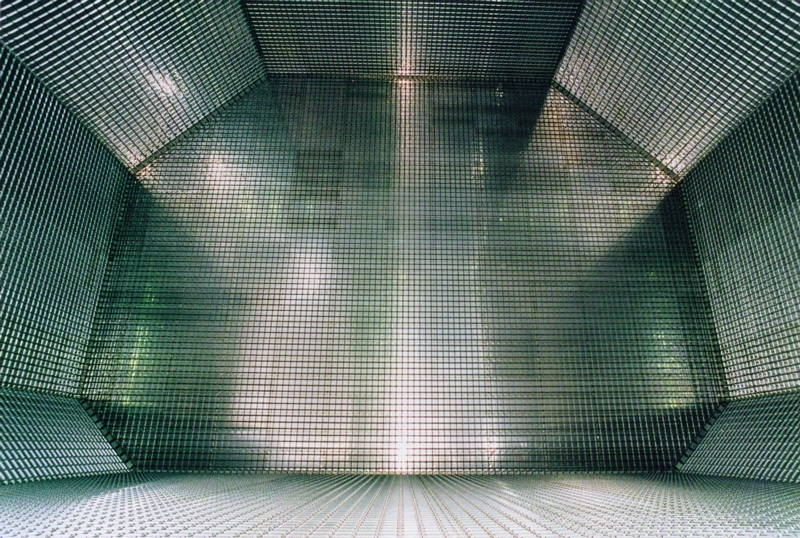
\includegraphics[width=.8\textwidth]{v5ch2-memb-tank-int}
\caption[Interior of a LNG tanker ship]{Interior of a LNG tanker ship. 
%A typical tank from one of two potential vendors is made of 
%four 40,000~m$^3$ compartments, 35~m high by 45~m wide. 
The tank shown is 24~m high by 35~m wide with interior grid-like 
corrugations on a 0.34~m pitch. By comparison, a single LBNF 
cryostat is %18887~m$^3$, 
14.0~m high by 15.1~m wide.}
\label{fig:memb-tank-int}
\end{figure}

\begin{figure}[htbp]
\centering
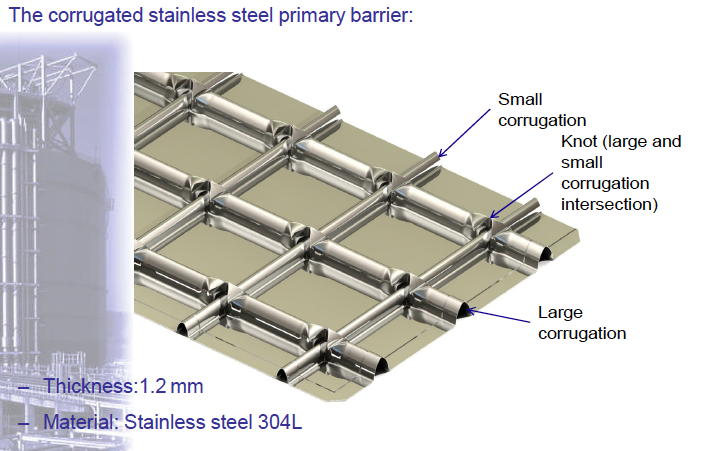
\includegraphics[width=.8\textwidth]{v5ch2-prim-barrier}
\caption[Primary membrane section]{Primary membrane section (courtesy GTT)}
\label{fig:prim-barrier}
\end{figure}

The advantages offered by the membrane design relative to a self-supporting cryostat are:
\begin{itemize}
%\item Lower cost due largely to the relative simplicity of a single cryogenic volume
\item Efficient use of the underground cavern volume due to its positioning 
close to the rock on floor and sides, which reduces the civil construction 
costs for the project
\item Higher ratio of usable (fiducial) mass to active (total) mass
\end{itemize}

Two membrane cryostat vendors have been 
identified. Those vendors are GTT (Gaztransport \& Technigaz) and 
IHI (Ishikawajima-Harima Heavy Industries). Each is technically capable 
of delivering a membrane cryostat that meets the design requirements for 
the LBNF. To provide clarity, only one vendor is represented here (GST 
system from GTT); this is for informational purposes only and should not 
be construed as preferring GTT over IHI. Nothing inherent in the IHI 
design changes the design approach. 

%ARUP has documented the two vendor products in their Fall 2011 report
%that updated previous designs specficially to the two-20-kT module 
%design at the 800L. 

\section{Design Parameters}
\label{sec:cryo-cryosys-params}

The requirements and parameters for the cryostat and cryogenic system 
design are within the LBNF requirement documentation~\cite{lar-fd-req}~\cite{lar-fd-req-traceback}  
and the parameter tables~\cite{lar-fd-params}, respectively. The 
overarching system requirements are to provide a high-purity, 
stable liquid argon environment for the TPC and to provide 
mechanical support for the TPC. For components that pass 
through the ullage (the vapor space above the LAr), no 
sources of reliquefaction may be present. Tables 
\ref{table:param-summ-LBNF} and \ref{table:cryo-reqs} 
offer a brief overview of parameters for a single 
cryostat of LBNF.

\begin{table}
\caption{Design parameters for one LBNF Cryostat}
\label{table:param-summ-LBNF}
 \begin{tabular}[htbp]{|l| p{8cm} |}
\hline
\textbf{Parameter} &  \textbf{Value} \\
\hline\hline
Cryostat Internal Volume &  13,107 m$^3$ \\
\hline
Total LAr Mass & 17.1 kton \\
\hline
Cryostat Inside Depth & 14.0 m \\
\hline
Cryostat Inside Width & 15.1 m \\
\hline
Cryostat Inside Length & 62.0 m  \\
\hline
Cryostat Outside Height & 16.62 m \\
\hline
Cryostat Outside Width & 18.72 m \\
\hline
Cryostat Outside Length & 65.62 m \\
\hline
Insulation &  Reinforced Polyurethane of 80~cm thickness; \\
           &  two (inner/outer) layers around secondary \\
           &  containment (40~cm per each layer) \\ 
\hline
Primary Membrane (GTT Design) & 1.2 mm thick type 304L stainless steel \\
                              & with corrugations on 340 mm $\times$ 503 mm \\
                       & rectangular pitch\\
\hline
Secondary Containment (GTT Design) & $\approx$ 0.07 mm thick aluminum between \\ 
                            & fiberglass cloth; overall thickness is \\
                            & 0.8 mm located between insulation layers \\
\hline
External Vapor Barrier Thickness & 10 mm \\
(Steel Plates)                   &       \\
\hline
External Support Structure Thickness & 1.0 m (Steel) \\
On Sides & \\
\hline
External Support Structure Thickness & 0.5 m (Steel) \\
Top and Bottom & \\
\hline
LAr Temperature & 88.3 $\pm$ 1 K \\
\hline
Minimum LAr Depth (Liquid Head) & 13.2 m \\
\hline
Ullage Operating Pressure & 130 mbarg (range: 50$-$200 mbarg) \\
\hline
Pressure at Bottom & 1,948 mbarg \\
\hline 
Cryostat Design Pressure & 350 mbarg \\
\hline
\end{tabular} 
\end{table}

% BN Jan 20 2012 changed Table to reflect 4850L

\begin{table}
\caption{Summary of parameters for membrane cryostat at the 4850L (the bottom of the Ross shaft)} 
\label{table:cryo-reqs}
\begin{tabular}[htbp]{| p{0.4\textwidth}|p{0.6\textwidth}|}
\hline 
\textbf{Property} & \textbf{Reference-Design Cryostat}\\
\hline\hline
Personnel Access to Cavern & Ross shaft\\
\hline
Equipment Transport to Cavern & Ross shaft, Yates shaft for long items \\
\hline
Construction Access to Pit & From above highbay \\
\hline
Type of Crane in Cavern & Mobile construction \\
\hline
Base & Steel structure \\
\hline
Side Walls & Steel structure \\
\hline
Heating System & Redundant/replaceable electric system \\
\hline
Roof & Pre-fabricated steel truss modules with lower steel plate \\
\hline
Vapor Barrier & Steel plates  \\
\hline
Insulation/Secondary Barrier/ & GST system by GTT \\
Membrane & \\
\hline
TPC & Individual 2.3 m $\times$ 6.0 m frames lowered through \\
    & 2.0 m $\times$ 4.0 m roof hatch. Assembled within \\
    & cryostat and suspended by hangers passing \\
    & through the roof. \\
\hline
LAr Containment System & Full Containment: Membrane/Secondary Barrier/ \\
                       & Steel Frame \\
\hline
\end{tabular} 
\end{table}


%%%%%%%%%%%%%%%%%%%%%%%%%%%%%%%%%%%%%%%%%%%%%%%%%%%%%%%%%%%%%%%%%%%%%%



\nomenclature{ADC}{analog-to-digital converter}
\nomenclature{APA}{anode plane assembly}
\nomenclature{APD}{avalanche photodiodes}
\nomenclature{ArgoNeuT}{Mini LArTPC Exposure to Fermilab's NuMI Beam}
\nomenclature{ASIC}{application-specific integrated circuit}
\nomenclature{BGR}{band-gap reference}
\nomenclature{CAD}{computer-aided design}  
\nomenclature{CDF}{one of two decommissioned collider detectors at Fermilab's Tevatron, along with D-Zero}  
\nomenclature{CF}{conventional facilities} 
\nomenclature{CFD}{computerized fluid dynamics} 
\nomenclature{CPA}{cathode plane assembly}
\nomenclature{DAQ}{data acquisition}
\nomenclature{DCM}{data concentrator module}
\nomenclature{DC}{direct current}
\nomenclature{DCM}{Data concentrator modules}
\nomenclature{D-Zero}{one of two decommissioned collider detectors at Fermilab's Tevatron, along with CDF}
\nomenclature{EM}{electromagnetic}
\nomenclature{ENC}{equivalent noise charge}
\nomenclature{ESH}{Environment, Safety and Health}
\nomenclature{FEM}{front-end module}
\nomenclature{FESHM}{Fermilab's ES\&H Manual}
\nomenclature{FFT}{Fast Fourier Transform}
\nomenclature{FIRUS}{Fire and Utilities; Fermilab site-wide, high-reliability, remote monitoring system used to monitor building fire panels and various utilities throughout the lab}
\nomenclature{FLARE}{Fermilab Liquid Argon Experiments}
\nomenclature{FPGA}{field-programmable gate array}
\nomenclature{FR-4}{flame resistant 4}
\nomenclature{FSE}{field-shaping electrode}
\nomenclature{GAr}{gaseous argon}
\nomenclature{GLACIER}{NASA's General Laboratory Active Cryogenic International Space Station Experiment Refrigerator}
\nomenclature{LNGS}{Gran Sasso National Laboratory}
\nomenclature{G10/FR4}{a fire rated electrical-grade dielectric made with and epoxy material reinforced with a woven fiberglass mat}
\nomenclature{GTT}{Gaztransport \& Technigaz}
\nomenclature{HSSD}{High Sensitivity Smoke Detection}
\nomenclature{HV}{high voltage}
\nomenclature{HVAC}{heating, ventilation and air conditioning}
\nomenclature{ICARUS}{Imaging Cosmic and Rare Underground Signals, experiment at the LNGS}
\nomenclature{INFN}{Istituto Nazionale della Fiscia Nucleare} 
\nomenclature{IHI}{Ishikawajima-Harima Heavy Industries}
\nomenclature{IT}{integration prototype}
\nomenclature{IU}{Indiana University}
\nomenclature{LANNDD}{Liquid Argon Neutrino and Nucleon Decay Detector}
\nomenclature{LAPD}{Liquid Argon Purity Demonstrator}
\nomenclature{LAr}{liquid argon}
\nomenclature{LAr1}{one-kiloton LAr prototype for LBNE's LAr-FD}
\nomenclature{LAr-FD}{LBNE's Liquid Argon Far Detector}
\nomenclature{LArSoft}{a reconstruction software package for LAr detectors}
\nomenclature{LArTPC}{liquid argon time projection chamber}
 \nomenclature{LBNE}{Long-Baseline Neutrino Experiment}
\nomenclature{LED}{light-emitting diode}
\nomenclature{LEM}{large electron multiplier}
\nomenclature{LEMO}{a push-pull connector made by the LEMO company in Switzerland}
\nomenclature{LHe}{liquid helium}
\nomenclature{LN}{liquid nitrogen, also written LN$_2$ and LN2}
\nomenclature{LNG}{liquefied natural gas}
\nomenclature{LOTO}{lockout/tagout; an OSHA safety practice }
\nomenclature{LPG}{liquefied petroleum gas}
\nomenclature{LVDS}{low-voltage differential signaling}
\nomenclature{MCT}{membrane cryostat test}
\nomenclature{MicroBooNE}{A 100-ton LArTPC located along Fermilab's Booster neutrino beamline }
\nomenclature{MINERvA}{A neutrino-scattering experiment that uses the NuMI beamline at Fermilab}
\nomenclature{MINOS}{Main Injector Neutrino Oscillation Search, a Fermilab experiment}
\nomenclature{MIP}{minimum ionizing particle}
\nomenclature{MIT}{Massachusetts Institute of Technology}
\nomenclature{MOS}{metal-oxide semiconductor}
\nomenclature{MOSFET}{metal-oxide-semiconductor field-effect transistor}
\nomenclature{MTU}{master timing unit}
\nomenclature{MUX}{multiplex}
\nomenclature{Bis-MSB}{1,4-bis[2-(2-methylphenyl)ethenyl]-benzene, a wavelength-shifting chemical}
\nomenclature{MTS}{Materials Test Stand}
\nomenclature{N or N2}{nitrogen}
\nomenclature{NASA}{National Aeronautics and Space Administration}
\nomenclature{NBTI}{negative bias temperature instability}
\nomenclature{NC}{neutral current}
\nomenclature{NICADD}{Northern Illinois Center for Accelerator and Detector Development NOvA}
\nomenclature{NIM}{Nuclear Instruments and Methods (journal)}
\nomenclature{NIST}{National Institute of Standards and Technology}
\nomenclature{NIST}{National Institute of Standards and Technology}
\nomenclature{NSF}{National Science Foundation}
\nomenclature{NOvA}{NuMI Off-Axis Neutrino Appearance experiment at Fermilab}
\nomenclature{OD}{outer diameter}
\nomenclature{ODH}{oxygen deficiency hazard}
\nomenclature{OPERA}{Oscillation Project with Emulsion-Racking Apparatus, at CERN and LNGS}
\nomenclature{OSHA}{Occupational Safety and Health Administration}
\nomenclature{PC}{personal computer}
\nomenclature{PC-4}{Fermilab building, Proton Center building number 4}
\nomenclature{PCI}{peripheral component interconnect}
\nomenclature{PDA}{photon detection assembly}
\nomenclature{PDE}{photon-detection efficiency}
\nomenclature{PE}{photo-electron}
\nomenclature{PLC}{programmable logic controller}
\nomenclature{PMT}{photomultiplier tube}
\nomenclature{PPE}{personnel protective equipment}
\nomenclature{PRV}{pressure-relief valve}
\nomenclature{QC}{quality control}
\nomenclature{RC}{resistive capacitive}
\nomenclature{ROOT}{An object oriented framework for large-scale data analysis developed at CERN}
\nomenclature{SCR}{silicon controlled rectifier}
\nomenclature{SDSTA}{South Dakota Science and Technology Authority}
\nomenclature{SIMOPS}{simultaneous operations study}
\nomenclature{SiPM}{Silicon photomultiplier}
\nomenclature{SM}{stress-migration}
\nomenclature{S/N}{signal-to-noise }
\nomenclature{SS}{stainless steel}
\nomenclature{TC}{thermal cycling}
\nomenclature{TDDB}{time-dependent dielectric breakdown}
\nomenclature{TDU}{timing distribution unit}
\nomenclature{TPB}{tetraphenyl butadiene, a wavelength shifting chemical}
\nomenclature{TPC}{Time Projection Chamber}
\nomenclature{USB}{universal serial bus}
\nomenclature{UV}{ultraviolet}
\nomenclature{VME}{a computer bus standard}
\nomenclature{VUV}{vacuum ultraviolet light}
\nomenclature{WARP}{Wimp Argon Program}
\nomenclature{WBS}{Work Breakdown Structure}
\nomenclature{WLS}{wavelength shifter}

\nomenclature{A}{ampere (also mA, kA)   }
\nomenclature{atm}{atmosphere}
\nomenclature{bar}{bar (also mbar, etc.)}
\nomenclature{barg}{bar gauge (deprecated per Wikipedia)}
\nomenclature{b}{barn, a measure of cross section; bit (also Mb, Gb, etc.)}
\nomenclature{B}{byte (also MB, GB, etc.)}
\nomenclature{Bq}{becquerel}
\nomenclature{C}{coulomb}
\nomenclature{cf}{cubic foot (also ft$^3$)}
\nomenclature{cfm}{cubic feet per meter (also ft$^3$/m)}
\nomenclature{Ci}{curie}
\nomenclature{eV}{electron-volt (also keV, MeV, GeV) }
\nomenclature{F}{farad (also pF, nF )}
\nomenclature{ft}{foot or feet }
\nomenclature{gal}{gallon}
\nomenclature{gpm}{gallons per minute (also gal/min)} 
\nomenclature{G}{gauss (also mG) or gradient (in magnets)}
\nomenclature{g}{gram (also mg, kg)}
\nomenclature{Hz}{hertz (s-1)}
\nomenclature{h}{hour}
\nomenclature{in}{inch }
\nomenclature{K}{kelvin} 
\nomenclature{l}{liter}
\nomenclature{m}{meter (also nm, micron, mm, cm, km) }
\nomenclature{min}{minute }
\nomenclature{MICA}{type of dielectric material used in capacitors}
\nomenclature{MS}{mega samples}
\nomenclature{N}{newton}
\nomenclature{NPO}{type of dielectric material used in capacitors}
\nomenclature{QFP}{quad flat pack}
\nomenclature{R}{roentgen}
\nomenclature{Pa}{pascal}
\nomenclature{psi}{pounds per square inch}
\nomenclature{rad}{radian (also mrad) }
\nomenclature{s}{second (also ns, $\mu$s, ms) }
\nomenclature{scfm}{standard cubic foot per minute }
\nomenclature{SHV}{safe high voltage, a type of HV cable connector}
\nomenclature{t}{ton}
\nomenclature{T}{Tesla}
\nomenclature{V}{volt (also mV, kV, MV)}
\nomenclature{VA}{volt-ampere (also mVA, kVA, MVA)}
\nomenclature{VAC}{Volts alternating current (also mVAC, kVAC)}
\nomenclature{VUV}{vacuum ultraviolet}
\nomenclature{W}{watt (also mW, kW, MW) }
\nomenclature{yd}{yard }
